In this section, we will provide an overview of the concept of \textit{Software-Defined Perimeters (SDP)} and their
role in network security.
Next, we will discuss the concept of \textit{Intrusion Detection Systems (IDSs)}, the available datasets, and their role
in the context of \textit{SDPs}.
Finally, we will also discuss the basics of \textit{Adversarial Machine Learning (AML)} and its potential for
exploitation in cyberattacks.
This information will provide the necessary context for the subsequent sections of this paper.

\subsection{Software-Defined Perimeters}\label{subsec:software-defined-perimeters}

The \textit{Software-Defined Perimeter (SDP)} is a security framework developed by the Cloud Security Alliance (CSA) to
dynamically protect networks~\cite{Koilpillai2020, Kumar2019}.
The \textit{Software-Defined Perimeter} framework was adapted from the \textit{Global Information Grid (GIG) Black Core}
initiative proposed by the USA Department of Defense (DoD)~\cite{Enterprise2007}.
The CSA modified the generalized DoD workflow for commercial use and aligned it with National Institute of Standards
and Technology (NIST) security controls.
The \textit{SDP} follows a strategy based on the \textit{Zero Trust} security model, where the identity of the device or
application that will initiate the communication is verified and authenticated before granting access to the
infrastructure~\cite{rose2020zero}.

In this model, there is a clear separation between its two main components (\textit{PDP} and \textit{PEP}),
which operate in the control plane and data plane respectively.
The \textit{Policy Decision Point (PDP)} includes trust and policy engines where authorization and access
decisions are made based on the information provided by the \textit{Policy Enforcement Point (PEP)}.

The architecture of SDP frameworks consists of three main components (see Figure~\ref{fig:sdp}).

\begin{figure*}
    \centering
    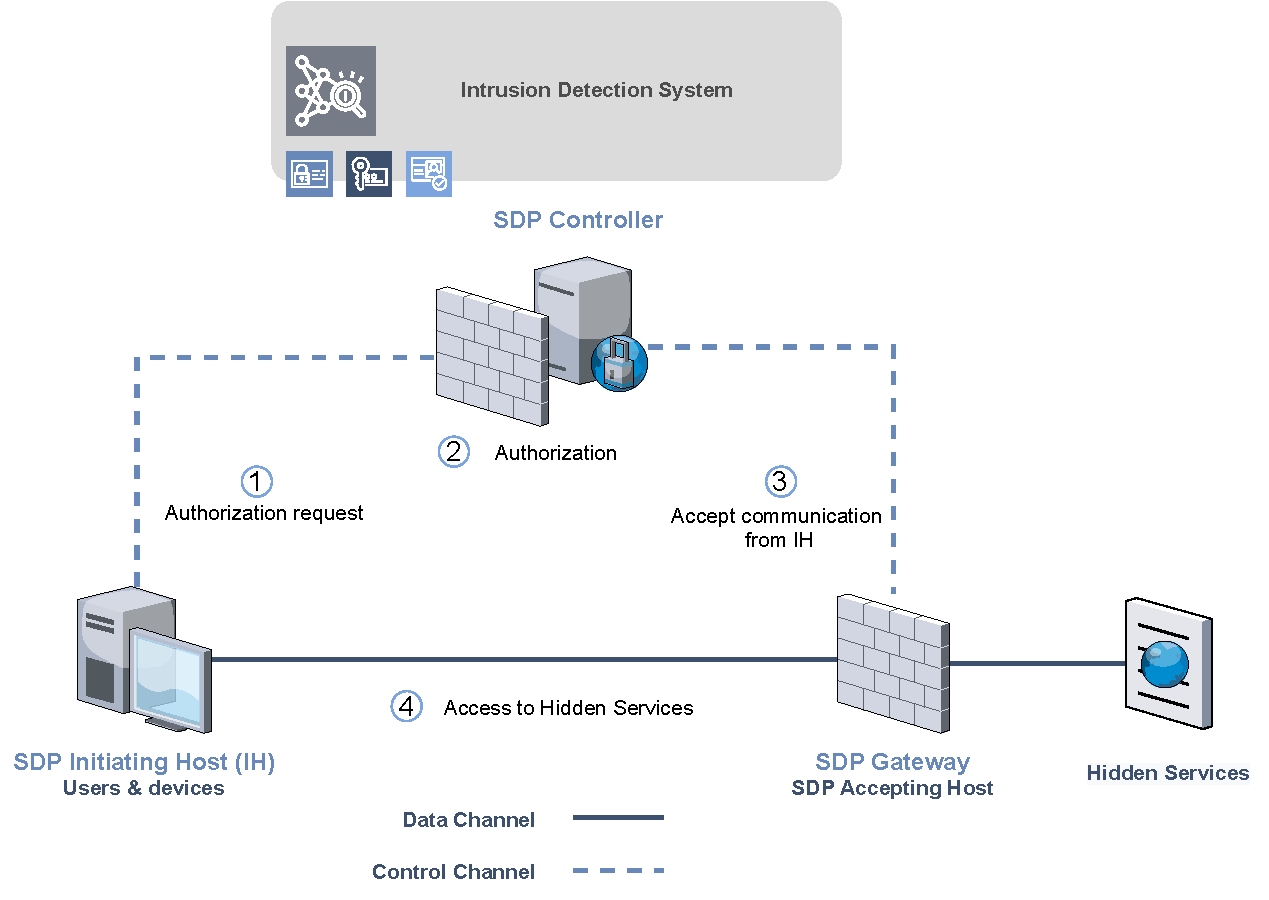
\includegraphics[width=.7\textwidth]{Figures/SDP}
    \caption{\label{fig:sdp} \textit{Software-Defined Perimeter} architecture~\cite{CSAZeroTrust2020}}
\end{figure*}


\subsubsection{SDP Controller}
The \textit{SDP Controller} is the central component of the \textit{SDP} framework and plays a crucial role in the
exchange of control messages.
It acts as a trusted agent between the \textit{SDP Initiating Host} and the backend security controls.
The \textit{SDP Controller} includes tasks for device identification and authentication, as well as determining which
programs or services are authorized for each device ~\cite{Koilpillai2020, Kumar2019}.
These tasks are crucial for the proper functioning of \textit{Intrusion Detection Systems (IDS)}, which are used to
identify and alert on unauthorized access or malicious activity within the network.

\subsubsection{SDP Initiating Host}
The \textit{SDP Initiating Host} is the device that initiates the connection to the backend security controls.
This device is responsible for sending the control messages to the \textit{SDP Controller} and for receiving the
authorization response from the \textit{SDP Controller} ~\cite{Koilpillai2020, Kumar2019}.
Once the authentication is completed, a mutual \textit{TLS tunnel} is created that connects the client (IH) to the
service or application for which it has authentication.

\subsubsection{SDP Accepting Host or Gateway}
\textit{Accepting Hosts} are the devices that are instructed to accept certain authorized services or applications.
The \textit{SDP Accepting Host} is protected by a firewall that allows only the authorized services or applications to
communicate with the \textit{SDP Initiating Host} ~\cite{Koilpillai2020, Kumar2019}.


\subsection{Intrusion Detection Systems}\label{subsec:intrusion-detection-systems}
\textit{Intrusion Detection Systems (IDS)} are security technologies designed to detect and alert on unauthorized
access or malicious activity within a network.
They are an important tool in protecting against cyber threats, such as malware, viruses, and hacking attempts.
\textit{IDSs} can operate in real-time, analyzing network traffic as it occurs, or they can be configured to analyze
logs or other stored data.
They use a variety of techniques to detect intrusions, such as analyzing network traffic patterns, examining system
logs, and looking for known malicious activity indicators.
\textit{IDSs} play a critical role in maintaining the security and integrity of a network, and are commonly used in
conjunction with other security measures such as firewalls and antivirus software.

\textit{Machine Learning (ML)} techniques have increasingly been used in \textit{IDSs} in recent
years~\cite{abdallah2022intrusion, thakkar2020review, maseer2021benchmarking} due to their ability to analyze large
amounts of data and identify complex patterns that might not be easily detected by traditional rule-based approaches.
\textit{ML-based IDSs} are capable of learning from past data and adapting to new patterns of behavior, which makes
them more effective at detecting new and evolving threats.
Additionally, \textit{ML} can be used to improve the accuracy and efficiency of \textit{IDSs} by reducing the number of
false positives and false negatives.

\subsection{Datasets overview}\label{subsec:datasets-overview}

\textit{Intrusion Detection Systems} datasets are an important resource for evaluating and benchmarking the performance
of \textit{IDSs}.
This datasets are typically collections of labeled examples of normal and abnormal network traffic, which are used to
train and test the accuracy and effectiveness of \textit{IDSs}.
There are several datasets available, each with its own characteristics and strengths.
In this part, we will review some of the most popular datasets and discuss their key features and uses.

\subsubsection{CIC-IDS2017}
The \textit{CIC-IDS2017} dataset~\cite{CICIDS2017} was created in a simulated enterprise network environment and captures
network traffic data over a five-day period.
The data was collected to mimic the behavior of 25 users and contains approximately 80 significant
attributes~\cite{RING2019147}.
It is currently one of the most widely used \textit{IDS} datasets in modern literature and contains a high ratio of
benign to malicious examples (83\% vs 17\%).
It can be used individually or in conjunction with other datasets, as it accurately reflects the normal distribution of
benign and malicious traffic in a network \cite{Shroff2022}.

\subsubsection{CSE-CIC-IDS2018}
The \textit{CSE-CIC-IDS2018} dataset~\cite{CSE-CIC-IDS2018}, created by the Canadian Institute for Cybersecurity (CIC),
was collected in a simulated enterprise network environment using AWS resources in 2018.
It contains data on seven different attack types and has approximately 79 significant features .
The dataset includes data from over 450 devices, including servers, computers, and other devices, and is notable for
its large size and high level of realism \cite{pujari2022comparative}.
It is similar to the \textit{CIC-IDS2017} dataset in that it includes packet analysis of network traffic with
bidirectional flow, but is larger and more comprehensive.
As a result, it is widely used in the literature for evaluating and benchmarking IDSs \cite{pujari2022comparative}.

\subsubsection{CIC-DDoS2019}
The \textit{CIC-DDoS2019} dataset~\cite{CICDDoS2019} was created to address the lack of representation of all subtypes
of DDoS attacks in existing datasets.
While the dataset includes simulated network traffic, efforts were made to create realistic benign data.
It includes 13 types of DDoS attacks and has more than 80 significant features.
However, the dataset is heavily imbalanced, with 50,006,249 records of DDoS attacks and only 56,863 records of benign
traffic, making it difficult to use for training a model on both types of data \cite{RING2019147}.
It is therefore recommended to use this dataset in conjunction with other datasets, such as \textit{CIC-IDS2017} or
\textit{CSE-CIC-IDS2018}, to train a more robust model \cite{Shroff2022}.

\subsubsection{ADFA IDS - UNSW-NB15}
The \textit{UNSW-NB15} dataset~\cite{UNSW-NB15} was developed at the University of New South Wales (UNSW) in Canberra
by the Cyber Range laboratory.
It is notable for its use of raw network packets that are a hybrid of real normal activities and synthetic contemporary
attack behaviors.
The dataset includes nine attack types and a total of 49 features, and is correctly labeled \cite{RING2019147}.
Unlike many other \textit{IDS} datasets, the \textit{UNSW-NB15} dataset is well-balanced, making it an excellent choice
for training models.

\subsubsection{Unused datasets}
There are many other \textit{IDS} datasets, such as \textit{Darpa 1998/99}~\cite{darpa1999},
\textit{KDD 99}~\cite{KDDCUP99} or \textit{NSL-KDD}~\cite{KDDCUP99}, which have not been used in this project.
The \textit{Darpa 1998/99} and \textit{KDD 99} datasets are no longer commonly used for evaluating and benchmarking
\textit{IDS} due to their outdated nature.
These datasets were created in the late 1990s and early 2000s, and do not accurately reflect the current landscape of
network threats and behaviors.
In particular, the \textit{KDD 99} dataset has been criticized for its high rate of false positives and its lack of
realism, which makes it less useful for testing the performance of modern \textit{IDS}~\cite{hugh2000, KDDFaults}.

On the other hand, datasets such as \textit{UNSW-NB15} and \textit{CIC-IDS2017} are more widely used due to their
larger size, greater realism, and more balanced distribution of benign and malicious examples .

\subsection{Adversarial Machine Learning}\label{subsec:adversarial-machine-learning}

\textit{Adversarial Machine Learning (AML)} refers to the use of \textit{Machine Learning} techniques to deceive or
mislead models.
According to the taxonomy of the attack and with Emiliano de Cristofaro \cite{de2020overview}, they can be classified into poisoning attacks, evasion attacks, inference
attacks, and extraction attacks.

\begin{itemize}
    \item \textbf{Poisoning attacks}: This attack involves modifying the training data in a way that causes the model to perform
    poorly on specific types of inputs.
    These attacks can be targeted at specific data points or can be more general, affecting the model's overall
    performance.
    Poisoning attacks can be difficult to detect, as the modified data can be indistinguishable from normal data.

    \item \textbf{Evasion attacks}: This attack involves generating inputs that are specifically designed to evade detection by the
    model.
    These inputs, known as adversarial examples, are modified versions of normal inputs that have been slightly
    perturbed in a way that is not easily noticeable to humans, but can cause the model to misclassify them.
    Evasion attacks can be conducted using a variety of techniques, such as gradient-based optimization or \textit{ML}.

    \item \textbf{Inference attacks}: This attack consists of inverting the sense of the information in a Machine Learning model. 
    The purpose is to get information from the model, which was not intended to be shared.
    There are three main sub-types of inference attack,
    \textit{Membership Inference Attack (MIA)} which is to discover whether or not a piece of data has been used in training,
    \textit{Property Inference Attack (PIA)} which attempts to infer model parameters and statistics,
    and Data Reconstruction which attempts to replicate the training samples.


    \item \textbf{Extraction attacks}: This attack is based on obtaining data from Machine Learning models.
    It uses a series of requests to the model, which allows it to intuit or predict the behavior of a model.
    These attacks can be easily detected as they need to send many suspicious requests.
    This type of attack it is intended to reveal the inner workings of the model,
    once enough knowledge is obtained, the model can be replicated or profit can be made from this information.  


\end{itemize}

In the context of \textit{IDSs}, \textit{AML} can be used to attack the \textit{IDS} by generating adversarial examples
that are designed to evade detection.
These attacks can be difficult to defend against~\cite{kariyappa2020defending}, as they rely on the ability to generate
inputs that are specifically designed to deceive the \textit{IDS}.
Some of the most common evasion attacks types used in \textit{IDS} are the \textit{Model extraction attacks} and the
\textit{Input reconstruction attacks}.
In this context, and depending on the level of knowledge of the attacker, adversarial attacks can be classified into
three types:

\begin{itemize}
    \item \textbf{White-box attacks}: In a white-box attack, the attacker has complete access to all information about
    the ML-based \textit{IDS}, including the training data and learning model architecture, decision and parameters
    (gradient, loss function, etc.).
    This gives the attacker a significant advantage, but fortunately, this type of attack is generally not practical
    in most real-world situations.

    \item \textbf{Black-box attacks}: In a black-box attack, the attacker has no knowledge of the \textit{IDS} model
    architecture, parameters, or training data.

    \item \textbf{Gray-box attacks}: Gray-box attacks involve an attacker who has some level of knowledge about the
    ML-based \textit{IDS} and may have limited access to the training data.
    In this scenario, the attacker does not have complete information about the system, but has enough information to
    attack it and cause it to fail.
    This type of attack is considered more realistic because it takes into account the fact that an attacker may
    have partial knowledge of the system they are targeting.
\end{itemize}

It is worth noting that in academic literature, the term ``black-box attacks'' is sometimes used to refer to
``gray-box attacks''.
In this article, we use the terms ``gray/black-box'' to refer specifically to the type of gray-box attacks
described above, to distinguish them from the more general use of the term ``black-box'' in the literature.